\chapter{Noise generation and noise reduction}

\section{Problem statement}

In this problem, you are required to write a program to generate different types
of random noises started from the Uniform noise and Gaussian noise. \\
And then add some of these noises to the circuit image and investigate the different
mean filters and order statistics as the textbook did at pages 344-352.

\section{Python implementation}

Usage:~\textbf{problem4.py [-h] (--uniform | --gaussian) [--histogram] \\}
\textbf{[--arithmetic] [--geometric] [--harmonic] [--contraharmonic] [-q Q]} \\
\textbf{[--median] [--max] [--min] [--midpoint] [--alpha] [-d D]} \\
\textbf{image\_path} \\\\
Use \textbf{python problem4.py -h} to see the help.

\pagebreak
\section{Gaussian noise}

\subsection{Noise generation and histogram}

\textbf{python problem4.py --gaussian circuit.tif}

\begin{figure}[!htb]\centering
    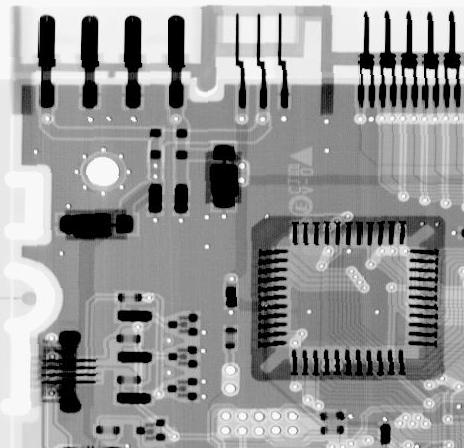
\includegraphics[width=0.6\linewidth]{./images/4/original.jpg}
    \caption{\small{Original image}}
\end{figure}

\begin{figure}[!htb]\centering
    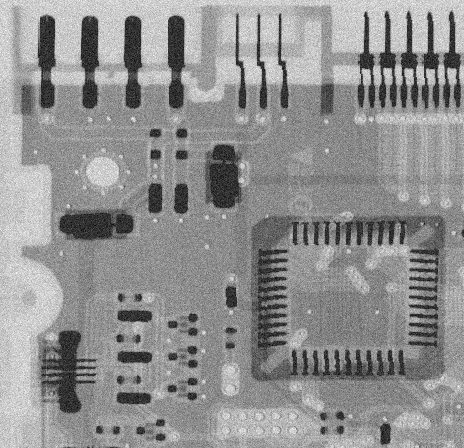
\includegraphics[width=0.6\linewidth]{./images/4/gaussian_noise.jpg}
    \caption{\small{Image + Gaussian noise ($\mu = 0, \sigma = 20$)}}\label{diagram:gaussian_noise}
\end{figure}


\pagebreak
\textbf{python problem4.py --gaussian --histogram circuit.tif}

\begin{figure}[!htb]\centering
    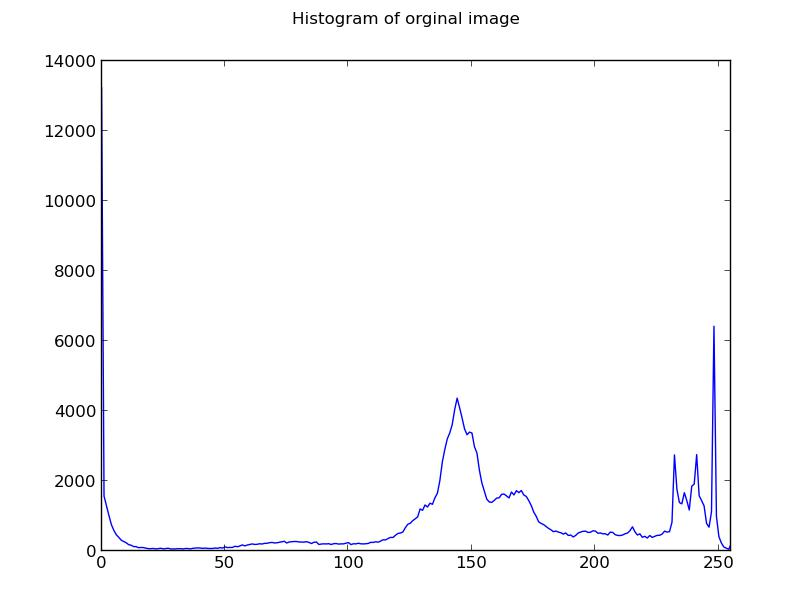
\includegraphics[width=0.7\linewidth]{./images/4/histogram_original.jpg}
    \caption{\small{Histogram of original image}}\label{diagram:histogram_original}
\end{figure}

\begin{figure}[!htb]\centering
    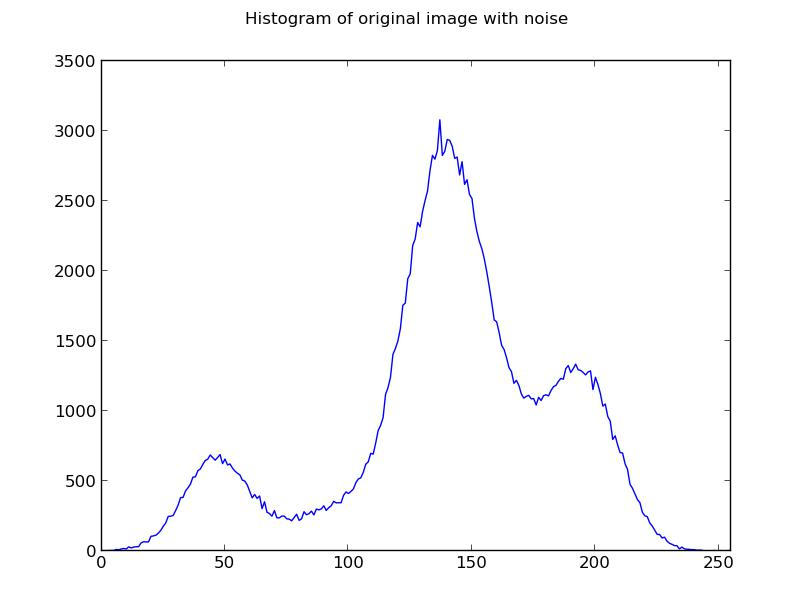
\includegraphics[width=0.7\linewidth]{./images/4/histogram_gaussian.jpg}
    \caption{\small{Histogram of image with Gaussian noise}}\label{diagram:histogram_gaussian}
\end{figure}


\pagebreak
\subsection{Noise reduction}

\subsubsection{Mean filters}

\begin{minipage}{\textwidth}
\textbf{python problem4.py --gaussian --arithmetic circuit.tif} \\
\textbf{python problem4.py --gaussian --geometric circuit.tif} \\
\end{minipage}

\begin{figure}[!htb]\centering
    \begin{minipage}{0.45\textwidth}
        \frame{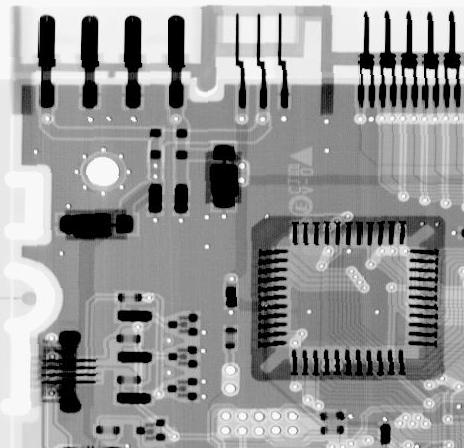
\includegraphics[width=\linewidth]{./images/4/original.jpg}}
        \caption{\small{Original image}}
    \end{minipage}
    \begin{minipage}{0.45\textwidth}
        \frame{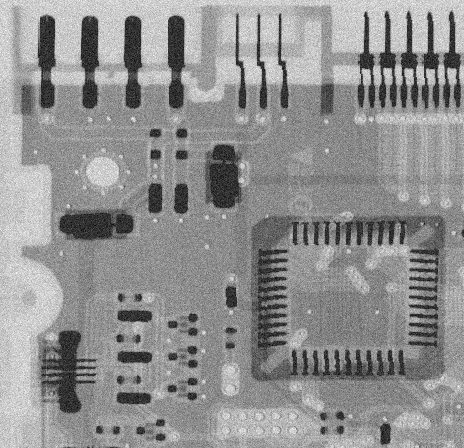
\includegraphics[width=\linewidth]{./images/4/gaussian_noise.jpg}}
        \caption{\small{Image + Gaussian}}
    \end{minipage}
\end{figure}

\begin{figure}[!htb]\centering
    \begin{minipage}{0.45\textwidth}
        \frame{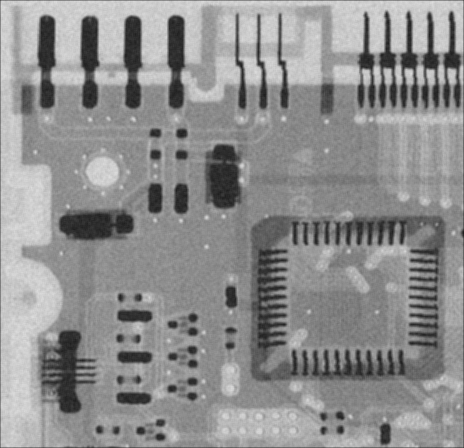
\includegraphics[width=\linewidth]{./images/4/gaussian_arithmetic.jpg}}
        \caption{\small{Arithmetic filter}}\label{diagram:gaussian_arithmetic}
    \end{minipage}
    \begin{minipage}{0.45\textwidth}
    \frame{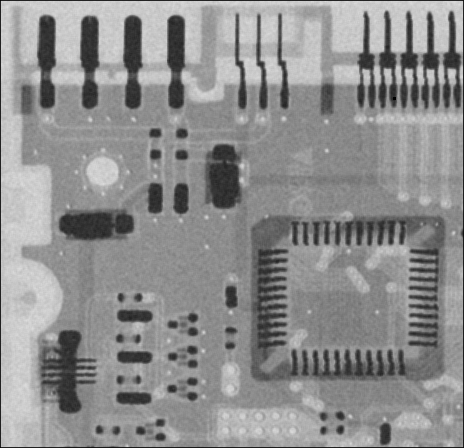
\includegraphics[width=\linewidth]{./images/4/gaussian_geometric.jpg}}
    \caption{\small{Geometric filter}}\label{diagram:gaussian_geometric}
    \end{minipage}
\end{figure}

\pagebreak
\begin{minipage}{\textwidth}
\textbf{python problem4.py --gaussian --harmonic circuit.tif} \\
\end{minipage}

\begin{figure}[!htb]\centering
    \begin{minipage}{0.45\textwidth}
        \frame{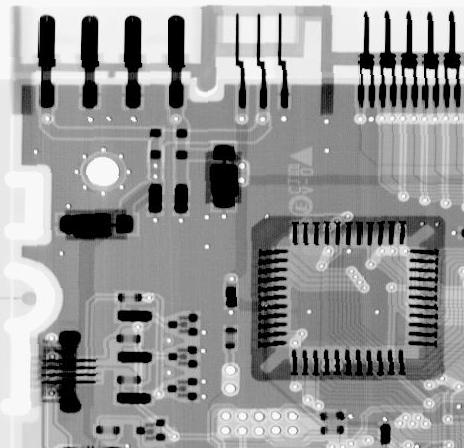
\includegraphics[width=\linewidth]{./images/4/original.jpg}}
        \caption{\small{Original image}}
    \end{minipage}
    \begin{minipage}{0.45\textwidth}
        \frame{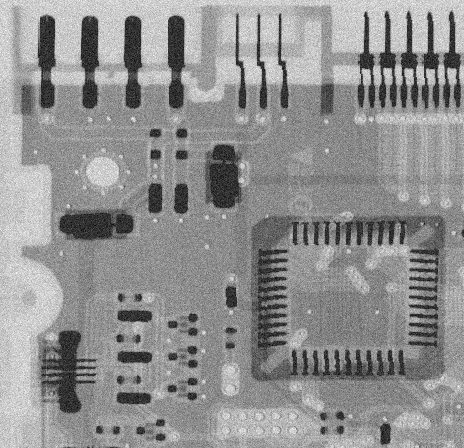
\includegraphics[width=\linewidth]{./images/4/gaussian_noise.jpg}}
        \caption{\small{Image + Gaussian}}
    \end{minipage}
\end{figure}

\begin{figure}[!htb]\centering
    \begin{minipage}{0.45\textwidth}
        \frame{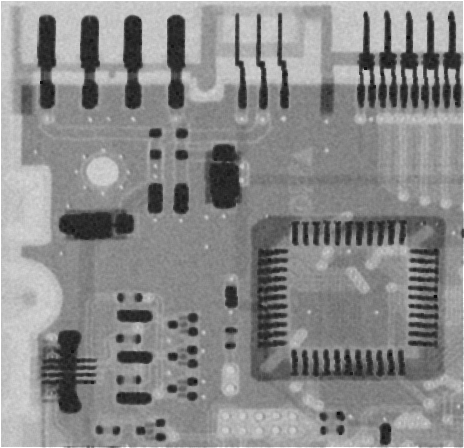
\includegraphics[width=\linewidth]{./images/4/gaussian_harmonic.jpg}}
        \caption{\small{Harmonic filter}}\label{diagram:gaussian_harmonic}
    \end{minipage}
\end{figure}

\pagebreak
\begin{minipage}{\textwidth}
\textbf{python problem4.py --gaussian --contraharmonic -q 1.5 circuit.tif} \\
\textbf{python problem4.py --gaussian --contraharmonic -q -1.5 circuit.tif} \\
\end{minipage}

\begin{figure}[!htb]\centering
    \begin{minipage}{0.45\textwidth}
        \frame{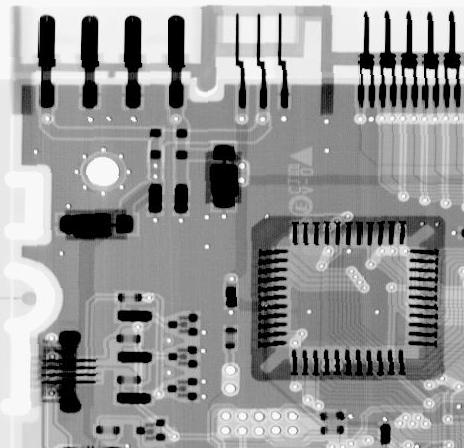
\includegraphics[width=\linewidth]{./images/4/original.jpg}}
        \caption{\small{Original image}}
    \end{minipage}
    \begin{minipage}{0.45\textwidth}
        \frame{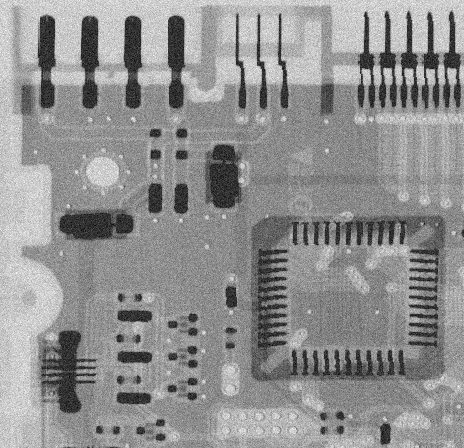
\includegraphics[width=\linewidth]{./images/4/gaussian_noise.jpg}}
        \caption{\small{Image + Gaussian}}
    \end{minipage}
\end{figure}

\begin{figure}[!htb]\centering
    \begin{minipage}{0.45\textwidth}
        \frame{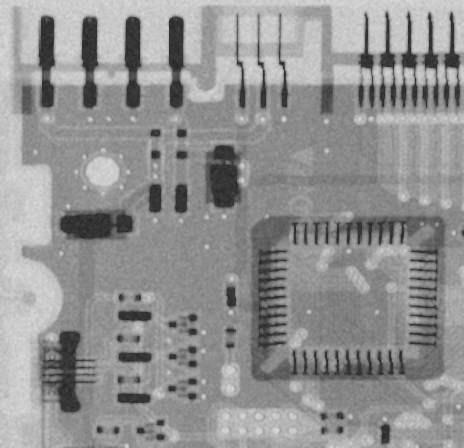
\includegraphics[width=\linewidth]{./images/4/gaussian_contraharmonic_1-5.jpg}}
        \caption{\small{Contra-harmonic filter (Q=1.5)}}\label{diagram:gaussian_contraharmonic_1_5}
    \end{minipage}
    \begin{minipage}{0.45\textwidth}
        \frame{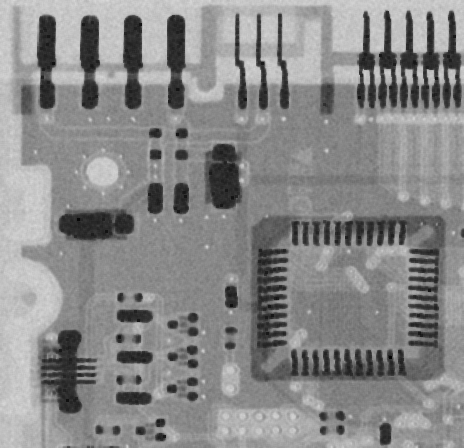
\includegraphics[width=\linewidth]{./images/4/gaussian_contraharmonic_-1-5.jpg}}
        \caption{\small{Contra-harmonic filter (Q=-1.5)}}\label{diagram:gaussian_contraharmonic_-1_5}
    \end{minipage}
\end{figure}


\pagebreak
\subsubsection{Order-Statistic filters}

\begin{minipage}{\textwidth}
\textbf{python problem4.py --gaussian --median circuit.tif} \\
\end{minipage}

\begin{figure}[!htb]\centering
    \begin{minipage}{0.45\textwidth}
        \frame{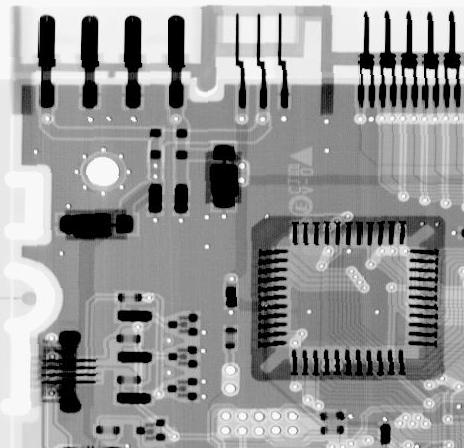
\includegraphics[width=\linewidth]{./images/4/original.jpg}}
        \caption{\small{Original image}}
    \end{minipage}
    \begin{minipage}{0.45\textwidth}
        \frame{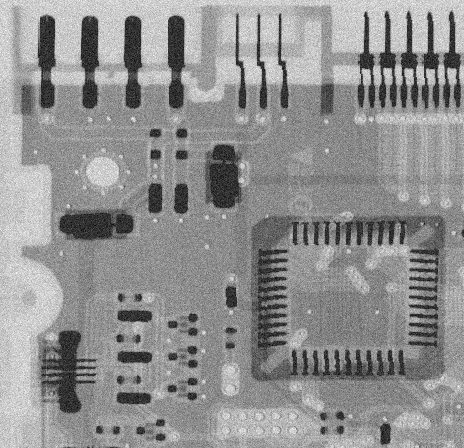
\includegraphics[width=\linewidth]{./images/4/gaussian_noise.jpg}}
        \caption{\small{Image + Gaussian}}
    \end{minipage}
\end{figure}

\begin{figure}[!htb]\centering
    \begin{minipage}{0.45\textwidth}
        \frame{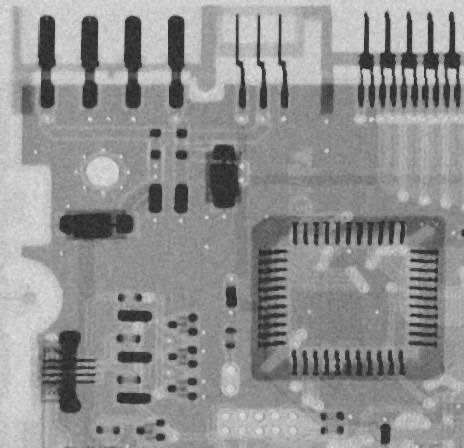
\includegraphics[width=\linewidth]{./images/4/gaussian_median.jpg}}
        \caption{\small{Median filter}}\label{diagram:gaussian_median}
    \end{minipage}
\end{figure}

\pagebreak
\begin{minipage}{\textwidth}
\textbf{python problem4.py --gaussian --max circuit.tif} \\
\textbf{python problem4.py --gaussian --min circuit.tif} \\
\end{minipage}

\begin{figure}[!htb]\centering
    \begin{minipage}{0.45\textwidth}
        \frame{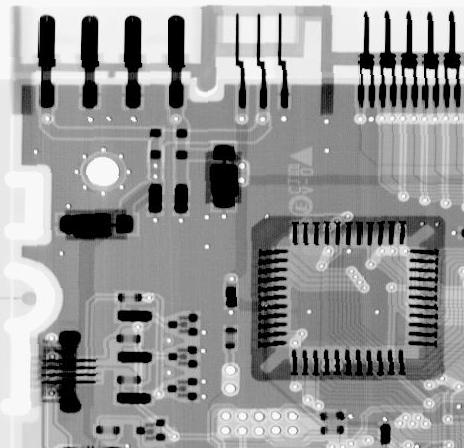
\includegraphics[width=\linewidth]{./images/4/original.jpg}}
        \caption{\small{Original image}}
    \end{minipage}
    \begin{minipage}{0.45\textwidth}
        \frame{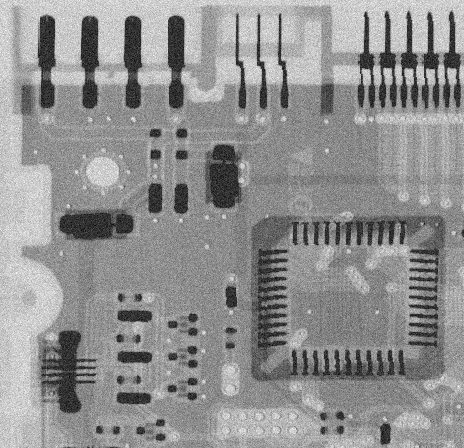
\includegraphics[width=\linewidth]{./images/4/gaussian_noise.jpg}}
        \caption{\small{Image + Gaussian}}
    \end{minipage}
\end{figure}

\begin{figure}[!htb]\centering
    \begin{minipage}{0.45\textwidth}
        \frame{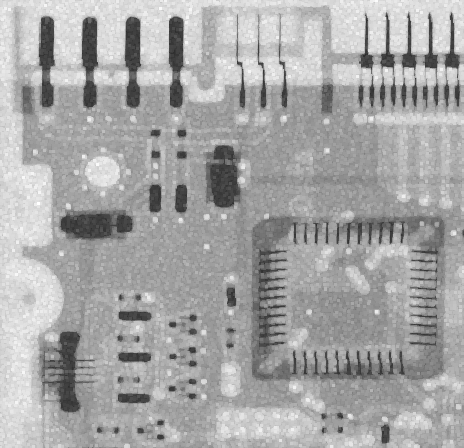
\includegraphics[width=\linewidth]{./images/4/gaussian_max.jpg}}
        \caption{\small{Max filter}}\label{diagram:gaussian_max}
    \end{minipage}
    \begin{minipage}{0.45\textwidth}
        \frame{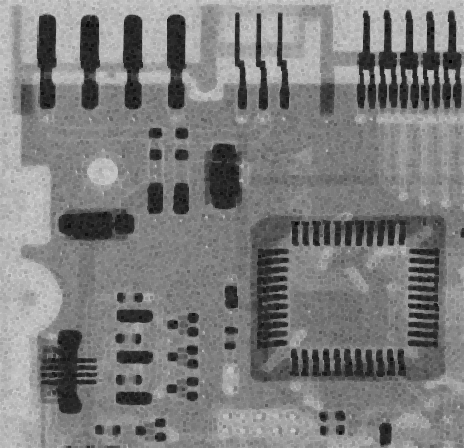
\includegraphics[width=\linewidth]{./images/4/gaussian_min.jpg}}
        \caption{\small{Min filter}}\label{diagram:gaussian_min}
    \end{minipage}
\end{figure}

\pagebreak
\begin{minipage}{\textwidth}
\textbf{python problem4.py --gaussian --midpoint circuit.tif} \\
\end{minipage}

\begin{figure}[!htb]\centering
    \begin{minipage}{0.45\textwidth}
        \frame{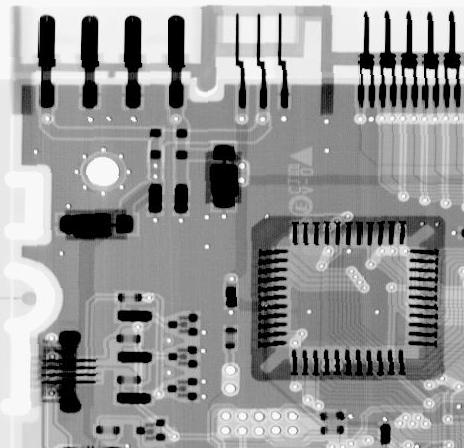
\includegraphics[width=\linewidth]{./images/4/original.jpg}}
        \caption{\small{Original image}}
    \end{minipage}
    \begin{minipage}{0.45\textwidth}
        \frame{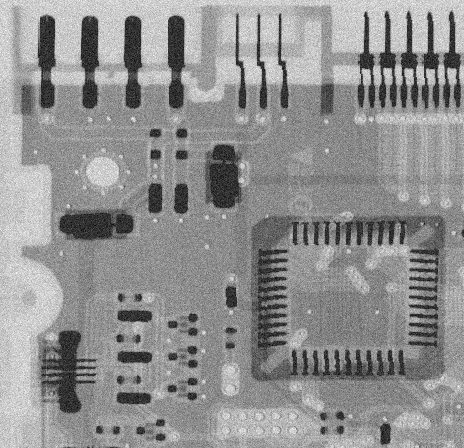
\includegraphics[width=\linewidth]{./images/4/gaussian_noise.jpg}}
        \caption{\small{Image + Gaussian}}
    \end{minipage}
\end{figure}

\begin{figure}[!htb]\centering
    \begin{minipage}{0.45\textwidth}
        \frame{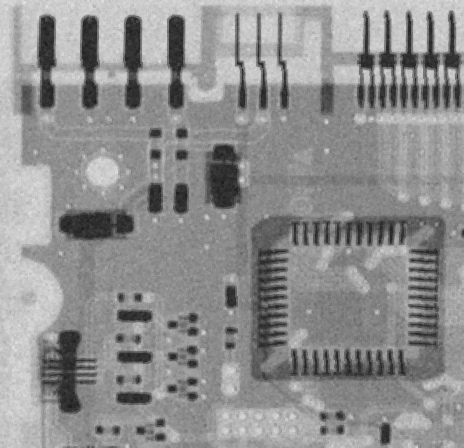
\includegraphics[width=\linewidth]{./images/4/gaussian_midpoint.jpg}}
        \caption{\small{Midpoint filter}}\label{diagram:gaussian_midpoint}
    \end{minipage}
\end{figure}


\pagebreak
\begin{minipage}{\textwidth}
\textbf{python problem4.py --gaussian --alpha -d 2 circuit.tif} \\
\textbf{python problem4.py --gaussian --alpha -d 4 circuit.tif} \\
\end{minipage}


\begin{figure}[!htb]\centering
    \begin{minipage}{0.45\textwidth}
        \frame{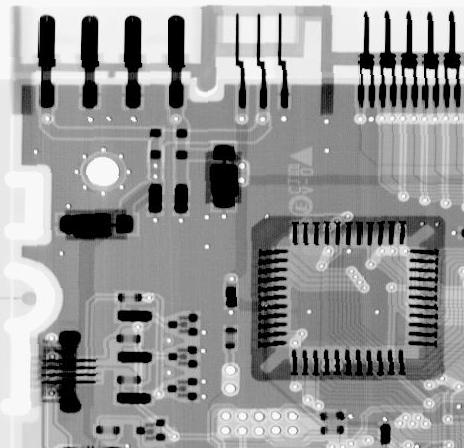
\includegraphics[width=\linewidth]{./images/4/original.jpg}}
        \caption{\small{Original image}}
    \end{minipage}
    \begin{minipage}{0.45\textwidth}
        \frame{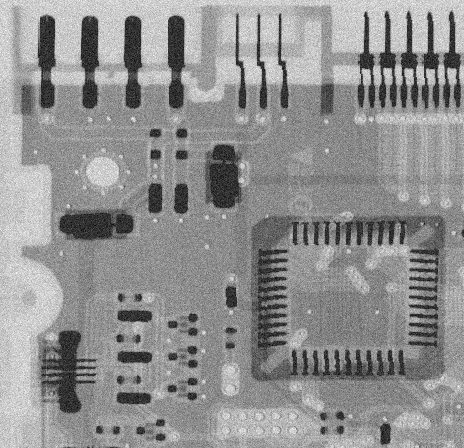
\includegraphics[width=\linewidth]{./images/4/gaussian_noise.jpg}}
        \caption{\small{Image + Gaussian}}
    \end{minipage}
\end{figure}

\begin{figure}[!htb]\centering
    \begin{minipage}{0.45\textwidth}
        \frame{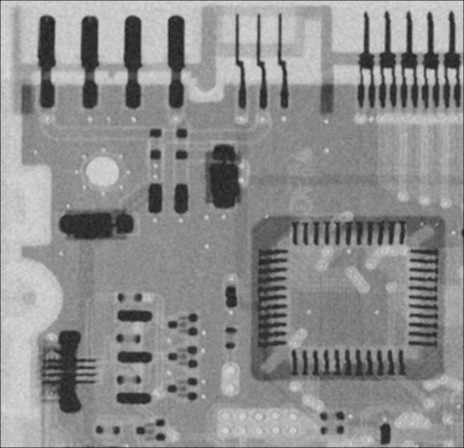
\includegraphics[width=\linewidth]{./images/4/gaussian_alpha_2.jpg}}
        \caption{\small{Alpha-trimmed filter \\(d = 2)}}\label{diagram:gaussian_alpha_2}
    \end{minipage}
    \begin{minipage}{0.45\textwidth}
        \frame{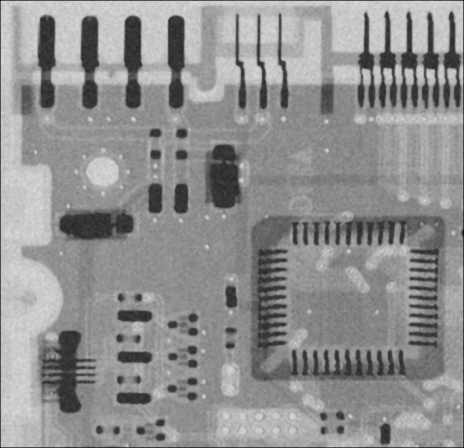
\includegraphics[width=\linewidth]{./images/4/gaussian_alpha_4.jpg}}
        \caption{\small{Alpha-trimmed filter \\(d = 4)}}\label{diagram:gaussian_alpha_4}
    \end{minipage}
\end{figure}


\pagebreak
\section{Uniform noise}

\subsection{Noise generation and histogram}

\textbf{python problem4.py --uniform circuit.tif}

\begin{figure}[!htb]\centering
    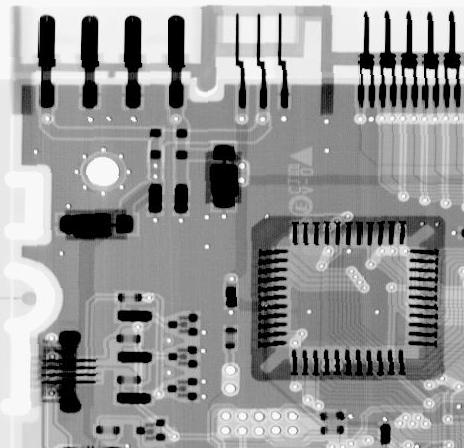
\includegraphics[width=0.6\linewidth]{./images/4/original.jpg}
    \caption{\small{Original image}}
\end{figure}

\begin{figure}[!htb]\centering
    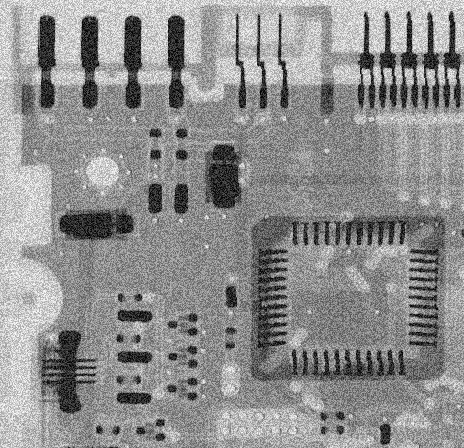
\includegraphics[width=0.6\linewidth]{./images/4/uniform_noise.jpg}
    \caption{\small{Image + Uniform noise (min = 0, max = 128)}}\label{diagram:uniform_noise}
\end{figure}


\pagebreak
\textbf{python problem4.py --uniform --histogram circuit.tif}

\begin{figure}[!htb]\centering
    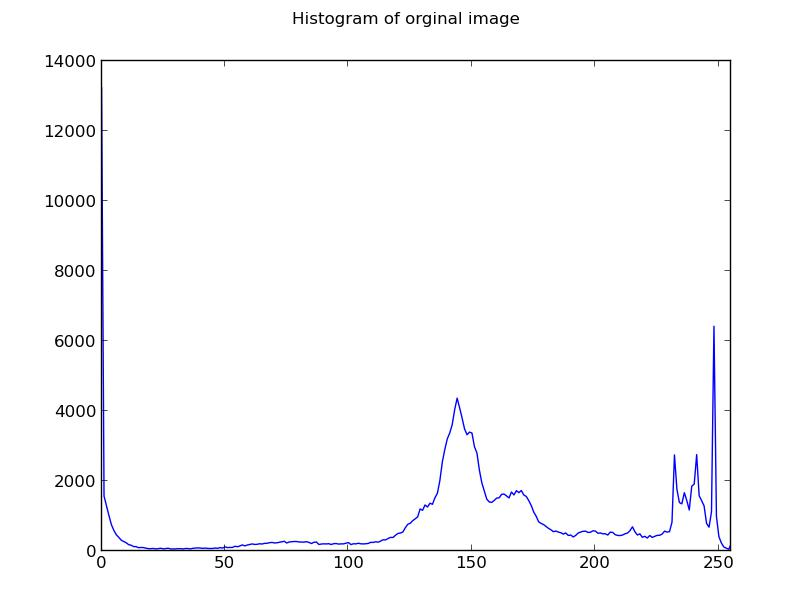
\includegraphics[width=0.7\linewidth]{./images/4/histogram_original.jpg}
    \caption{\small{Histogram of original image}}\label{diagram:histogram_original}
\end{figure}

\begin{figure}[!htb]\centering
    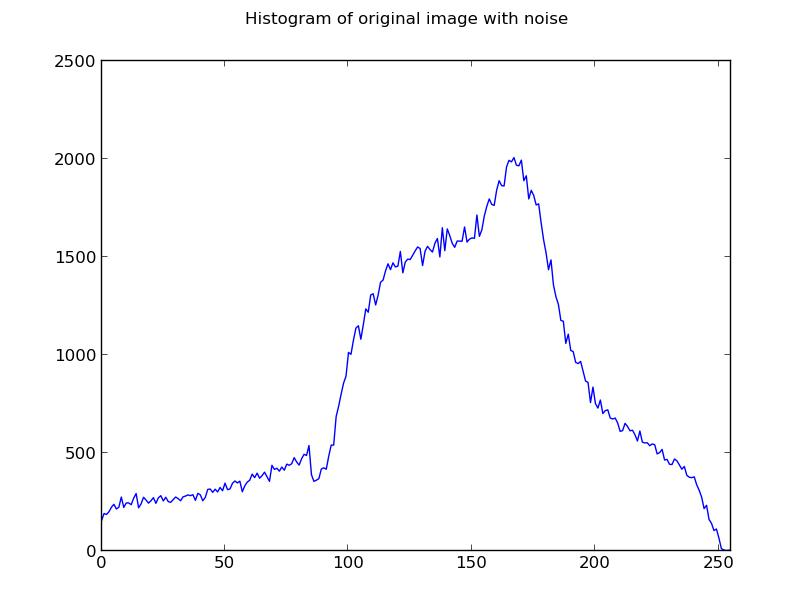
\includegraphics[width=0.7\linewidth]{./images/4/histogram_uniform.jpg}
    \caption{\small{Histogram of image with Uniform noise}}\label{diagram:histogram_uniform}
\end{figure}


\pagebreak
\subsection{Noise reduction}

\subsubsection{Mean filters}

\begin{minipage}{\textwidth}
\textbf{python problem4.py --uniform --arithmetic circuit.tif} \\
\textbf{python problem4.py --uniform --geometric circuit.tif} \\
\end{minipage}

\begin{figure}[!htb]\centering
    \begin{minipage}{0.45\textwidth}
        \frame{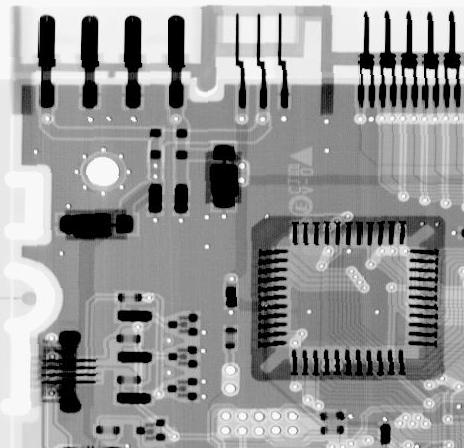
\includegraphics[width=\linewidth]{./images/4/original.jpg}}
        \caption{\small{Original image}}
    \end{minipage}
    \begin{minipage}{0.45\textwidth}
        \frame{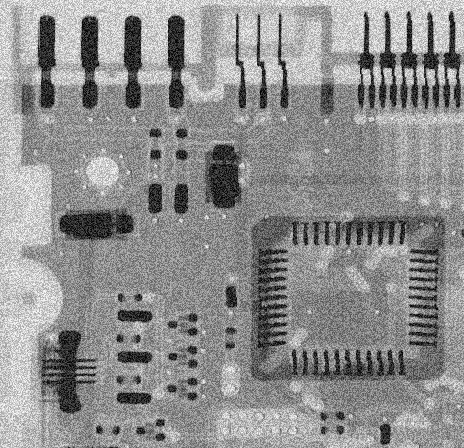
\includegraphics[width=\linewidth]{./images/4/uniform_noise.jpg}}
        \caption{\small{Image + Uniform}}
    \end{minipage}
\end{figure}

\begin{figure}[!htb]\centering
    \begin{minipage}{0.45\textwidth}
        \frame{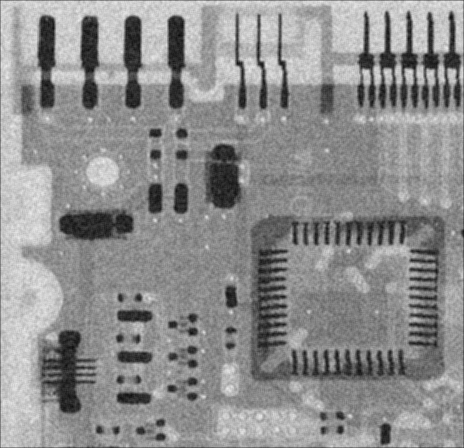
\includegraphics[width=\linewidth]{./images/4/uniform_arithmetic.jpg}}
        \caption{\small{Arithmetic filter}}\label{diagram:uniform_arithmetic}
    \end{minipage}
    \begin{minipage}{0.45\textwidth}
    \frame{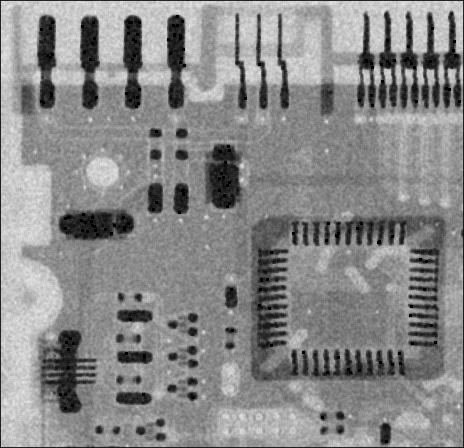
\includegraphics[width=\linewidth]{./images/4/uniform_geometric.jpg}}
    \caption{\small{Geometric filter}}\label{diagram:uniform_geometric}
    \end{minipage}
\end{figure}

\pagebreak
\begin{minipage}{\textwidth}
\textbf{python problem4.py --uniform --harmonic circuit.tif} \\
\end{minipage}

\begin{figure}[!htb]\centering
    \begin{minipage}{0.45\textwidth}
        \frame{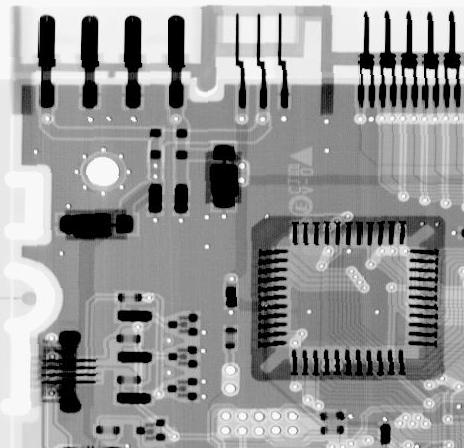
\includegraphics[width=\linewidth]{./images/4/original.jpg}}
        \caption{\small{Original image}}
    \end{minipage}
    \begin{minipage}{0.45\textwidth}
        \frame{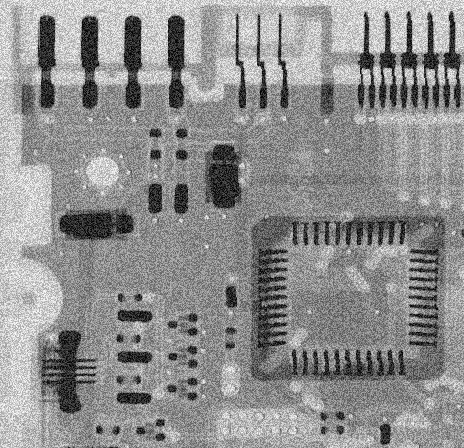
\includegraphics[width=\linewidth]{./images/4/uniform_noise.jpg}}
        \caption{\small{Image + Uniform}}
    \end{minipage}
\end{figure}

\begin{figure}[!htb]\centering
    \begin{minipage}{0.45\textwidth}
        \frame{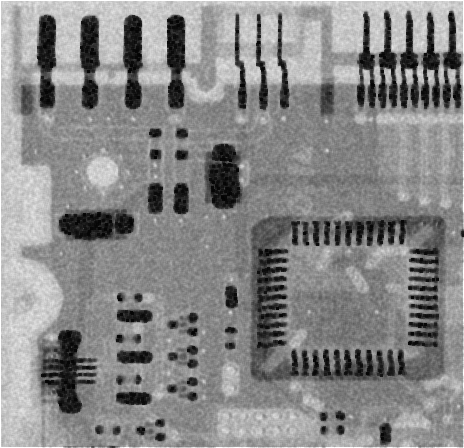
\includegraphics[width=\linewidth]{./images/4/uniform_harmonic.jpg}}
        \caption{\small{Harmonic filter}}\label{diagram:uniform_harmonic}
    \end{minipage}
\end{figure}

\pagebreak
\begin{minipage}{\textwidth}
\textbf{python problem4.py --uniform --contraharmonic -q 1.5 circuit.tif} \\
\textbf{python problem4.py --uniform --contraharmonic -q -1.5 circuit.tif} \\
\end{minipage}

\begin{figure}[!htb]\centering
    \begin{minipage}{0.45\textwidth}
        \frame{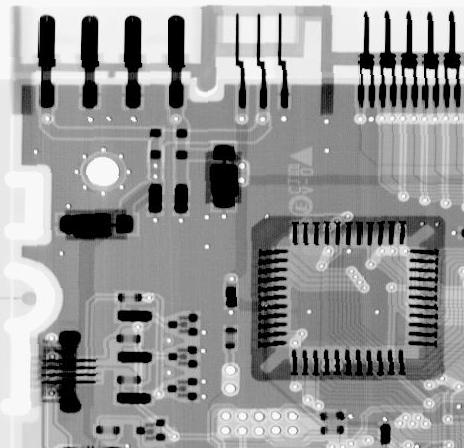
\includegraphics[width=\linewidth]{./images/4/original.jpg}}
        \caption{\small{Original image}}
    \end{minipage}
    \begin{minipage}{0.45\textwidth}
        \frame{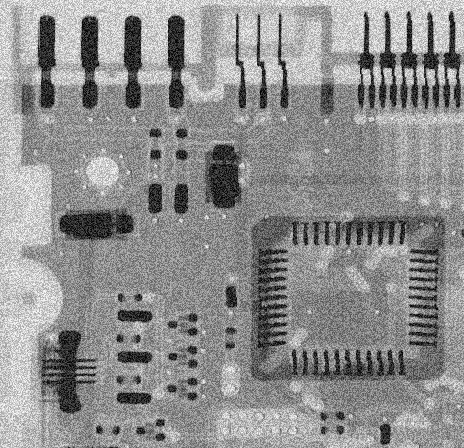
\includegraphics[width=\linewidth]{./images/4/uniform_noise.jpg}}
        \caption{\small{Image + Uniform}}
    \end{minipage}
\end{figure}

\begin{figure}[!htb]\centering
    \begin{minipage}{0.45\textwidth}
        \frame{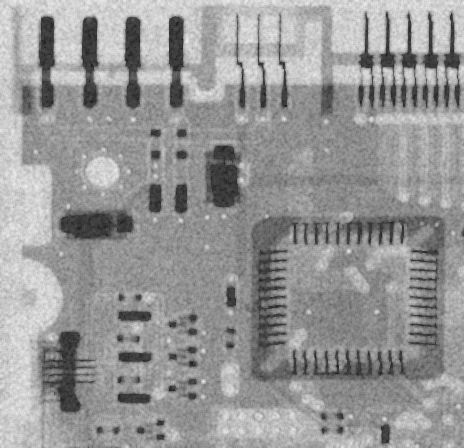
\includegraphics[width=\linewidth]{./images/4/uniform_contraharmonic_1-5.jpg}}
        \caption{\small{Contra-harmonic filter (Q=1.5)}}\label{diagram:uniform_contraharmonic_1_5}
    \end{minipage}
    \begin{minipage}{0.45\textwidth}
        \frame{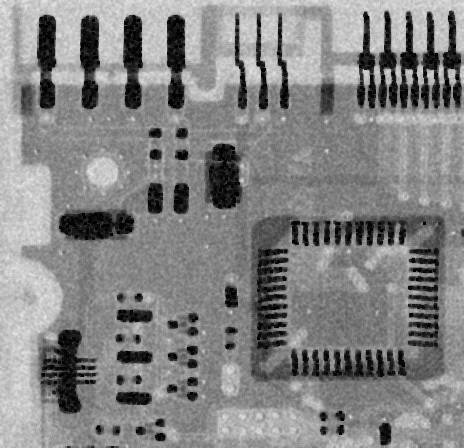
\includegraphics[width=\linewidth]{./images/4/uniform_contraharmonic_-1-5.jpg}}
        \caption{\small{Contra-harmonic filter (Q=-1.5)}}\label{diagram:uniform_contraharmonic_-1_5}
    \end{minipage}
\end{figure}


\pagebreak
\subsubsection{Order-Statistic filters}

\begin{minipage}{\textwidth}
\textbf{python problem4.py --uniform --median circuit.tif} \\
\end{minipage}

\begin{figure}[!htb]\centering
    \begin{minipage}{0.45\textwidth}
        \frame{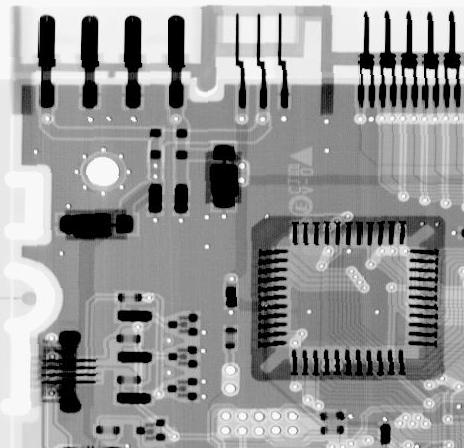
\includegraphics[width=\linewidth]{./images/4/original.jpg}}
        \caption{\small{Original image}}
    \end{minipage}
    \begin{minipage}{0.45\textwidth}
        \frame{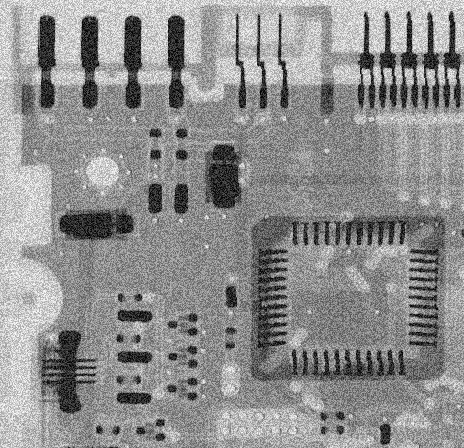
\includegraphics[width=\linewidth]{./images/4/uniform_noise.jpg}}
        \caption{\small{Image + Uniform}}
    \end{minipage}
\end{figure}

\begin{figure}[!htb]\centering
    \begin{minipage}{0.45\textwidth}
        \frame{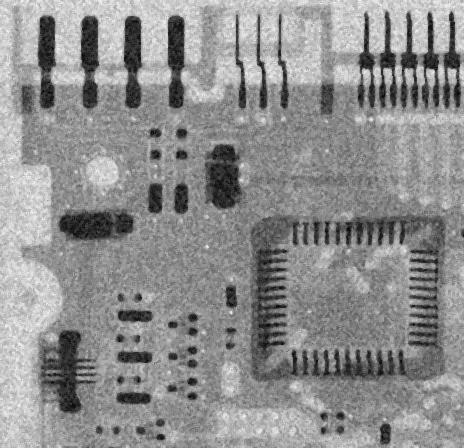
\includegraphics[width=\linewidth]{./images/4/uniform_median.jpg}}
        \caption{\small{Median filter}}\label{diagram:uniform_median}
    \end{minipage}
\end{figure}

\pagebreak
\begin{minipage}{\textwidth}
\textbf{python problem4.py --uniform --max circuit.tif} \\
\textbf{python problem4.py --uniform --min circuit.tif} \\
\end{minipage}

\begin{figure}[!htb]\centering
    \begin{minipage}{0.45\textwidth}
        \frame{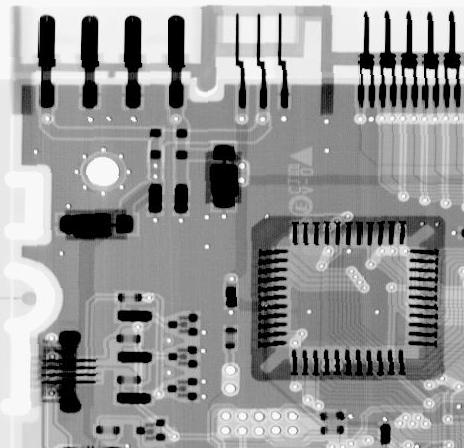
\includegraphics[width=\linewidth]{./images/4/original.jpg}}
        \caption{\small{Original image}}
    \end{minipage}
    \begin{minipage}{0.45\textwidth}
        \frame{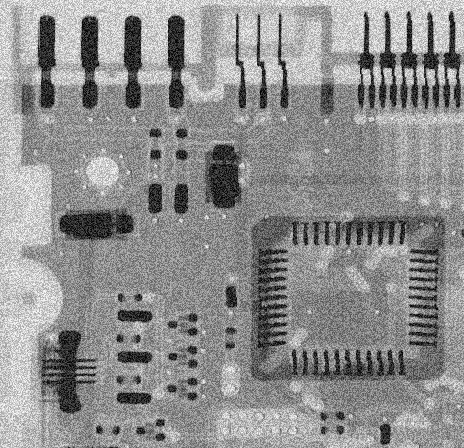
\includegraphics[width=\linewidth]{./images/4/uniform_noise.jpg}}
        \caption{\small{Image + Uniform}}
    \end{minipage}
\end{figure}

\begin{figure}[!htb]\centering
    \begin{minipage}{0.45\textwidth}
        \frame{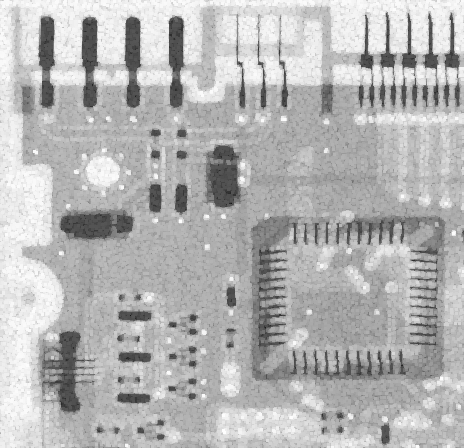
\includegraphics[width=\linewidth]{./images/4/uniform_max.jpg}}
        \caption{\small{Max filter}}\label{diagram:uniform_max}
    \end{minipage}
    \begin{minipage}{0.45\textwidth}
        \frame{\includegraphics[width=\linewidth]{./images/4/uniform_min.jpg}}
        \caption{\small{Min filter}}\label{diagram:uniform_min}
    \end{minipage}
\end{figure}

\pagebreak
\begin{minipage}{\textwidth}
\textbf{python problem4.py --uniform --midpoint circuit.tif} \\
\end{minipage}

\begin{figure}[!htb]\centering
    \begin{minipage}{0.45\textwidth}
        \frame{\includegraphics[width=\linewidth]{./images/4/original.jpg}}
        \caption{\small{Original image}}
    \end{minipage}
    \begin{minipage}{0.45\textwidth}
        \frame{\includegraphics[width=\linewidth]{./images/4/uniform_noise.jpg}}
        \caption{\small{Image + Uniform}}
    \end{minipage}
\end{figure}

\begin{figure}[!htb]\centering
    \begin{minipage}{0.45\textwidth}
        \frame{\includegraphics[width=\linewidth]{./images/4/uniform_midpoint.jpg}}
        \caption{\small{Midpoint filter}}\label{diagram:uniform_midpoint}
    \end{minipage}
\end{figure}


\pagebreak
\begin{minipage}{\textwidth}
\textbf{python problem4.py --uniform --alpha -d 2 circuit.tif} \\
\textbf{python problem4.py --uniform --alpha -d 4 circuit.tif} \\
\end{minipage}


\begin{figure}[!htb]\centering
    \begin{minipage}{0.45\textwidth}
        \frame{\includegraphics[width=\linewidth]{./images/4/original.jpg}}
        \caption{\small{Original image}}
    \end{minipage}
    \begin{minipage}{0.45\textwidth}
        \frame{\includegraphics[width=\linewidth]{./images/4/uniform_noise.jpg}}
        \caption{\small{Image + Uniform}}
    \end{minipage}
\end{figure}

\begin{figure}[!htb]\centering
    \begin{minipage}{0.45\textwidth}
        \frame{\includegraphics[width=\linewidth]{./images/4/uniform_alpha_2.jpg}}
        \caption{\small{Alpha-trimmed filter \\(d = 2)}}\label{diagram:uniform_alpha_2}
    \end{minipage}
    \begin{minipage}{0.45\textwidth}
        \frame{\includegraphics[width=\linewidth]{./images/4/uniform_alpha_4.jpg}}
        \caption{\small{Alpha-trimmed filter \\(d = 4)}}\label{diagram:uniform_alpha_4}
    \end{minipage}
\end{figure}
